\subsection{UC 25 - Eliminazione condivisione di un evento} \label{sec:UC25}

    \begin{itemize}
        \item \textbf{Attore principale}: MUA;
        \item \textbf{Descrizione}: il MUA deve poter eliminare una condivisione di un evento nel sistema;
        \item \textbf{Precondizioni}: il MUA sta usando la funzionalità di eliminazione di una condivisione;
        \item \textbf{Postcondizioni}: il sistema elimina la condivisione dell'evento con le informazioni fornite dal MUA;
        \item \textbf{Scenario principale}:
            \begin{enumerate}
                \item il MUA trasmette l'id dell'evento condiviso (\hyperref[sec:UC25.1]{UC 25.1});
                \item il MUA trasmette l'indirizzo e-mail a cui rimuovere la condivisione dell'evento (\hyperref[sec:UC25.2]{UC 25.2});
                \item il sistema rimuove la condivisione dell'evento;
            \end{enumerate}
        \item \textbf{Inclusioni}: nessuna;
        \item \textbf{Generalizzazioni}: nessuna;
        \item \textbf{Estensioni}: nessuna.
    \end{itemize}

    \begin{figure}[H]
        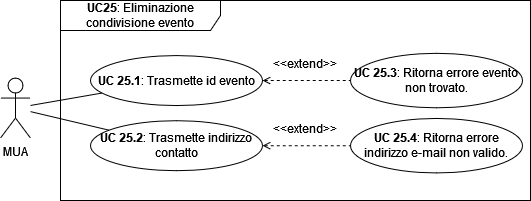
\includegraphics[width=0.85\textwidth]{sections/uc_imgs/UC25.png}
        \centering
        \caption{Diagramma sotto-casi UC 25}
    \end{figure}

    \subsubsection{UC 25.1 - Trasmette id evento} \label{sec:UC25.1}
    \begin{itemize}
        \item \textbf{Attore principale}: MUA;
        \item \textbf{Descrizione}: il MUA trasmette l'id dell'evento per eliminare la condivisione dell'evento;
        \item \textbf{Precondizioni}: il MUA sta usando la funzionalità di eliminazione condivisione di un evento;
        \item \textbf{Postcondizioni}: il sistema conosce l'id dell'evento di cui eliminare la condivisione;
        \item \textbf{Scenario principale}:
            \begin{enumerate}
                \item il MUA invia l'id dell'evento per eliminare la condivisione dell'evento;
            \end{enumerate}
        \item \textbf{Inclusioni}: nessuna;
        \item \textbf{Generalizzazioni}: nessuna;
        \item \textbf{Estensioni}:
            \begin{enumerate}[label=\alph*.]
                \item il sistema non riesce a eliminare la condivisione dell'evento perché l'id dell'evento fornito non è stato trovato:
                \begin{enumerate}[label=\arabic*.]
                    \item il sistema ritorna un errore al MUA di evento non trovato (\hyperref[sec:UC25.3]{UC 25.3}).
                \end{enumerate}
            \end{enumerate}
    \end{itemize}


    \subsubsection{UC 25.2 - Trasmette indirizzo contatto} \label{sec:UC25.2}
    \begin{itemize}
        \item \textbf{Attore principale}: MUA;
        \item \textbf{Descrizione}: il MUA trasmette l'indirizzo e-mail a cui togliere la condivisione al sistema;
        \item \textbf{Precondizioni}: il MUA sta usando la funzionalità di eliminazione condivisione di un evento;
        \item \textbf{Postcondizioni}: il sistema conosce l'indirizzo e-mail a cui rimuovere la condivisione;
        \item \textbf{Scenario principale}:
            \begin{enumerate}
                \item il MUA invia l'indirizzo e-mail a cui togliere la condivisione dell'evento al sistema;
                \item il sistema controlla che le informazioni ricevute rispettino il seguente requisito minimo:
                    \begin{itemize}
                        \item l'indirizzo e-mail non è una stringa vuota;
                    \end{itemize}
            \end{enumerate}
        \item \textbf{Inclusioni}: nessuna;
        \item \textbf{Generalizzazioni}: nessuna;
        \item \textbf{Estensioni}:
            \begin{enumerate}[label=\alph*.]
                \item il sistema non riesce ad eliminare la condivisione dell'evento perché l'indirizzo e-mail fornito non è valido:
                \begin{enumerate}[label=\arabic*.]
                    \item il sistema ritorna un errore al MUA di indirizzo e-mail non valido (\hyperref[sec:UC25.4]{UC 25.4}).
                \end{enumerate}
            \end{enumerate}
    \end{itemize}


\subsubsection{UC 25.3 - Ritorna errore evento non trovato} \label{sec:UC25.3}
    \begin{itemize}
        \item \textbf{Attore principale}: MUA;
        \item \textbf{Descrizione}: il sistema non riesce a eliminare la condivisione dell'evento perché l'evento non è stato trovato;
        \item \textbf{Precondizioni}: il MUA ha inviato l'id dell'evento a cui togliere la condivisione al sistema;
        \item \textbf{Postcondizioni}: il sistema non elimina la condivisione dell'evento, il MUA è stato notificato dell'errore;
        \item \textbf{Scenario principale}:
            \begin{enumerate}
                \item il sistema non trova l'evento con l'identificativo fornito dal MUA;
                \item il sistema non elimina la condivisione dell'evento e notifica il MUA dell'errore;
            \end{enumerate}
        \item \textbf{Inclusioni}: nessuna;
        \item \textbf{Generalizzazioni}: nessuna;
        \item \textbf{Estensioni}: nessuna.
    \end{itemize}

    \subsubsection{UC 25.4 - Ritorna errore indirizzo e-mail non valido} \label{sec:UC25.4}
    \begin{itemize}
        \item \textbf{Attore principale}: MUA;
        \item \textbf{Descrizione}: il sistema non riesce a eliminare la condivisione dell'evento perché l'indirizzo e-mail fornito non rispetta i requisiti;
        \item \textbf{Precondizioni}: il MUA ha inviato l'indirizzo e-mail a cui rimuovere la condivisione;
        \item \textbf{Postcondizioni}: il sistema non eliminazione la condivisione dell'evento, il MUA è stato notificato dell'errore;
        \item \textbf{Scenario principale}:
            \begin{enumerate}
                \item il sistema controlla la sintassi dell'indirizzo e-mail e trova un errore;
                \item il sistema non elimina la condivisione dell'evento e notifica il MUA dell'errore;
            \end{enumerate}
        \item \textbf{Inclusioni}: nessuna;
        \item \textbf{Generalizzazioni}: nessuna;
        \item \textbf{Estensioni}: nessuna.
    \end{itemize}
